\problemname{Bridge Building}
Rut, who hasn't learned to swim, wants to cross a river. Fortunately, a bridge is being constructed
over a section of the river, which can be represented as an $N \times M$ grid.
Every hour, a bridge segment is built on a tile that was previously covered by water. For example,
five bridge segments will have been built after five hours.
Rut has obtained a list of the positions of the first bridge segments to be built,
and she knows that she can cross the river when she can walk on the bridge from one side of the river
to the other without having to swim any part of the way.
She starts at row $0$ and wants to reach row $N-1$.
These two rows each have a landmass that she can use to walk along the entire river.
She can move between tiles that are not covered by water by moving up, down, right, or left.
She now wants to know if the given bridge segments are enough to cross, and if so, how many hours
she needs to wait before the bridge is sufficiently completed for her to be able to reach the other side.


\begin{figure}[h]
  \centering
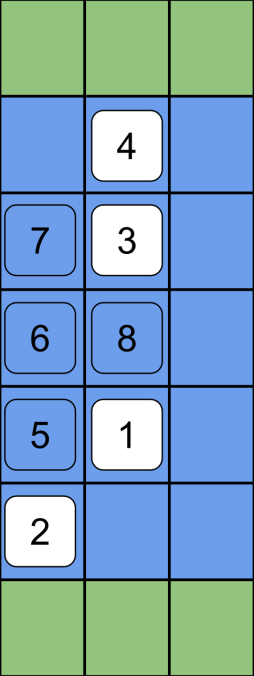
\includegraphics[width=0.2\textwidth]{brobygge_sample.png}
\quad
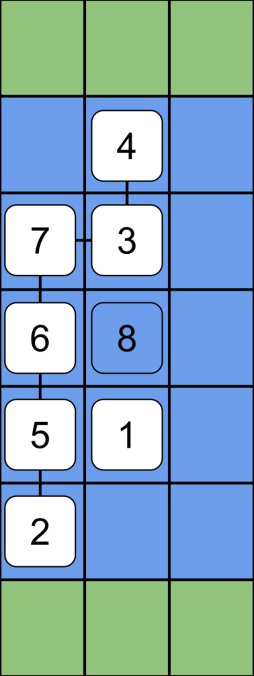
\includegraphics[width=0.2\textwidth]{brobygge_sample2.png}
  \caption{Illustration of sample 1 after 4 and 7 hours. Only after 7 hours will there be a path to the other side.}
\end{figure}


\section*{Input}
The first line of input contains three integers $N, M$ ($3 \le N, M \le 10^9$), and $T$ ($1 \le T \le 10^5$),
the number of rows and columns in the grid, and the number of bridge segments to be built, respectively.

This is followed by $T$ lines, where the $i$-th line contains two integers $R$ ($1 \le R \le N-2$) and $C$ ($0 \le C \le M-1$),
the row and column where a tile is completed in the $i$-th hour. Note that in this problem, row $0$ is the bottom row.

\section*{Output}
If Rut can cross the river, print an integer: the minimum number of hours Rut needs to wait for
the bridge to be sufficiently completed to walk to the other side. Otherwise, print ``nej'' (no).

\section*{Points}
Your solution will be tested on several test case groups.
To get the points for a group, it must pass all the test cases in the group.

\noindent
\begin{tabular}{| l | l | p{12cm} |}
  \hline
  \textbf{Group} & \textbf{Point value} & \textbf{Constraints} \\ \hline
  $1$    & $10$      & $N \le 4$ \\ \hline
  $2$    & $20$      & $N, M \le 50$ \\ \hline
  $3$    & $30$      & $N, M \le 1000$ \\ \hline
  $4$    & $15$      & $T \le 2000$ \\ \hline
  $5$    & $25$      & No additional constraints. \\ \hline
\end{tabular}

%\section*{Samples}
